\documentclass{beamer}
\usetheme{default}
\usepackage{chemformula}
\usepackage[super,sort&compress,comma]{natbib}

\title{Post-Christmas Update}
\author{Ben Goldmann}
\date{\today}

\usepackage{caption}
\captionsetup[figure]{labelformat=empty}
\captionsetup[table]{labelformat=empty}

\begin{document}

\begin{frame}
\titlepage
\end{frame}

\begin{frame}
\frametitle{Initial vs Refitted}

\begin{figure}
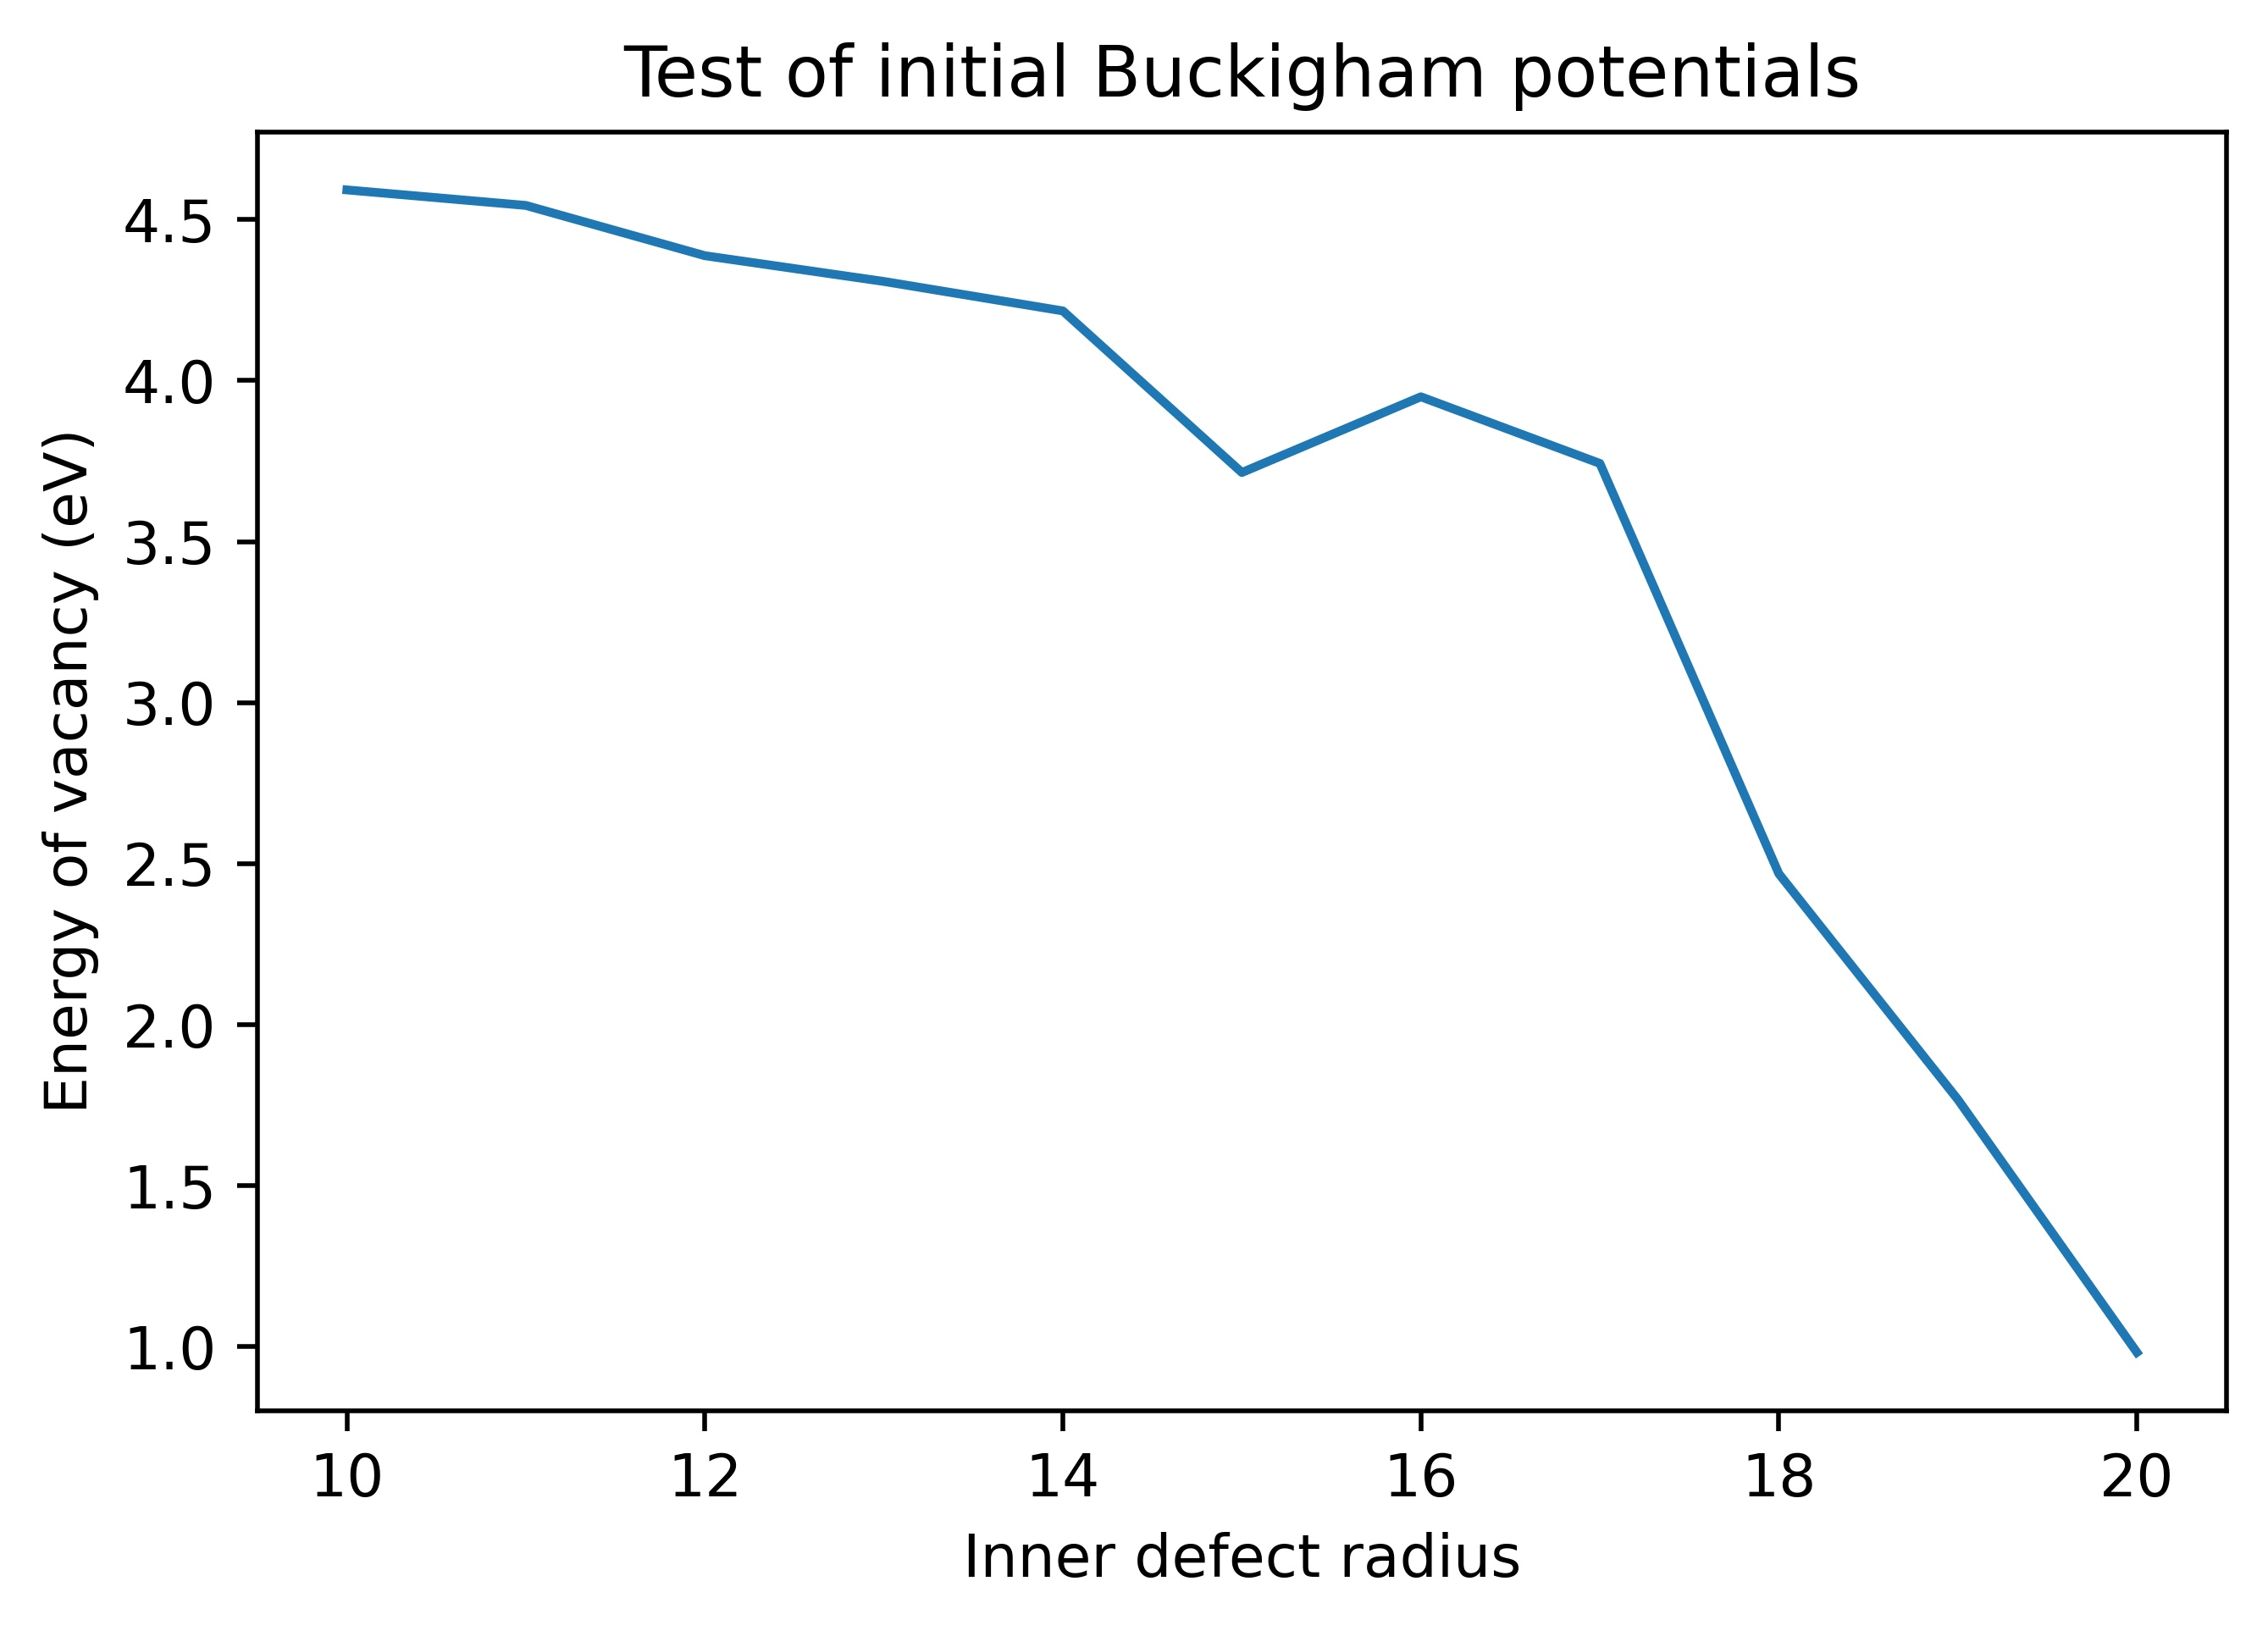
\includegraphics[width=0.5\textwidth]{/home/ben/Documents/gulp_calcs/0_summary/initial_test.jpg}%
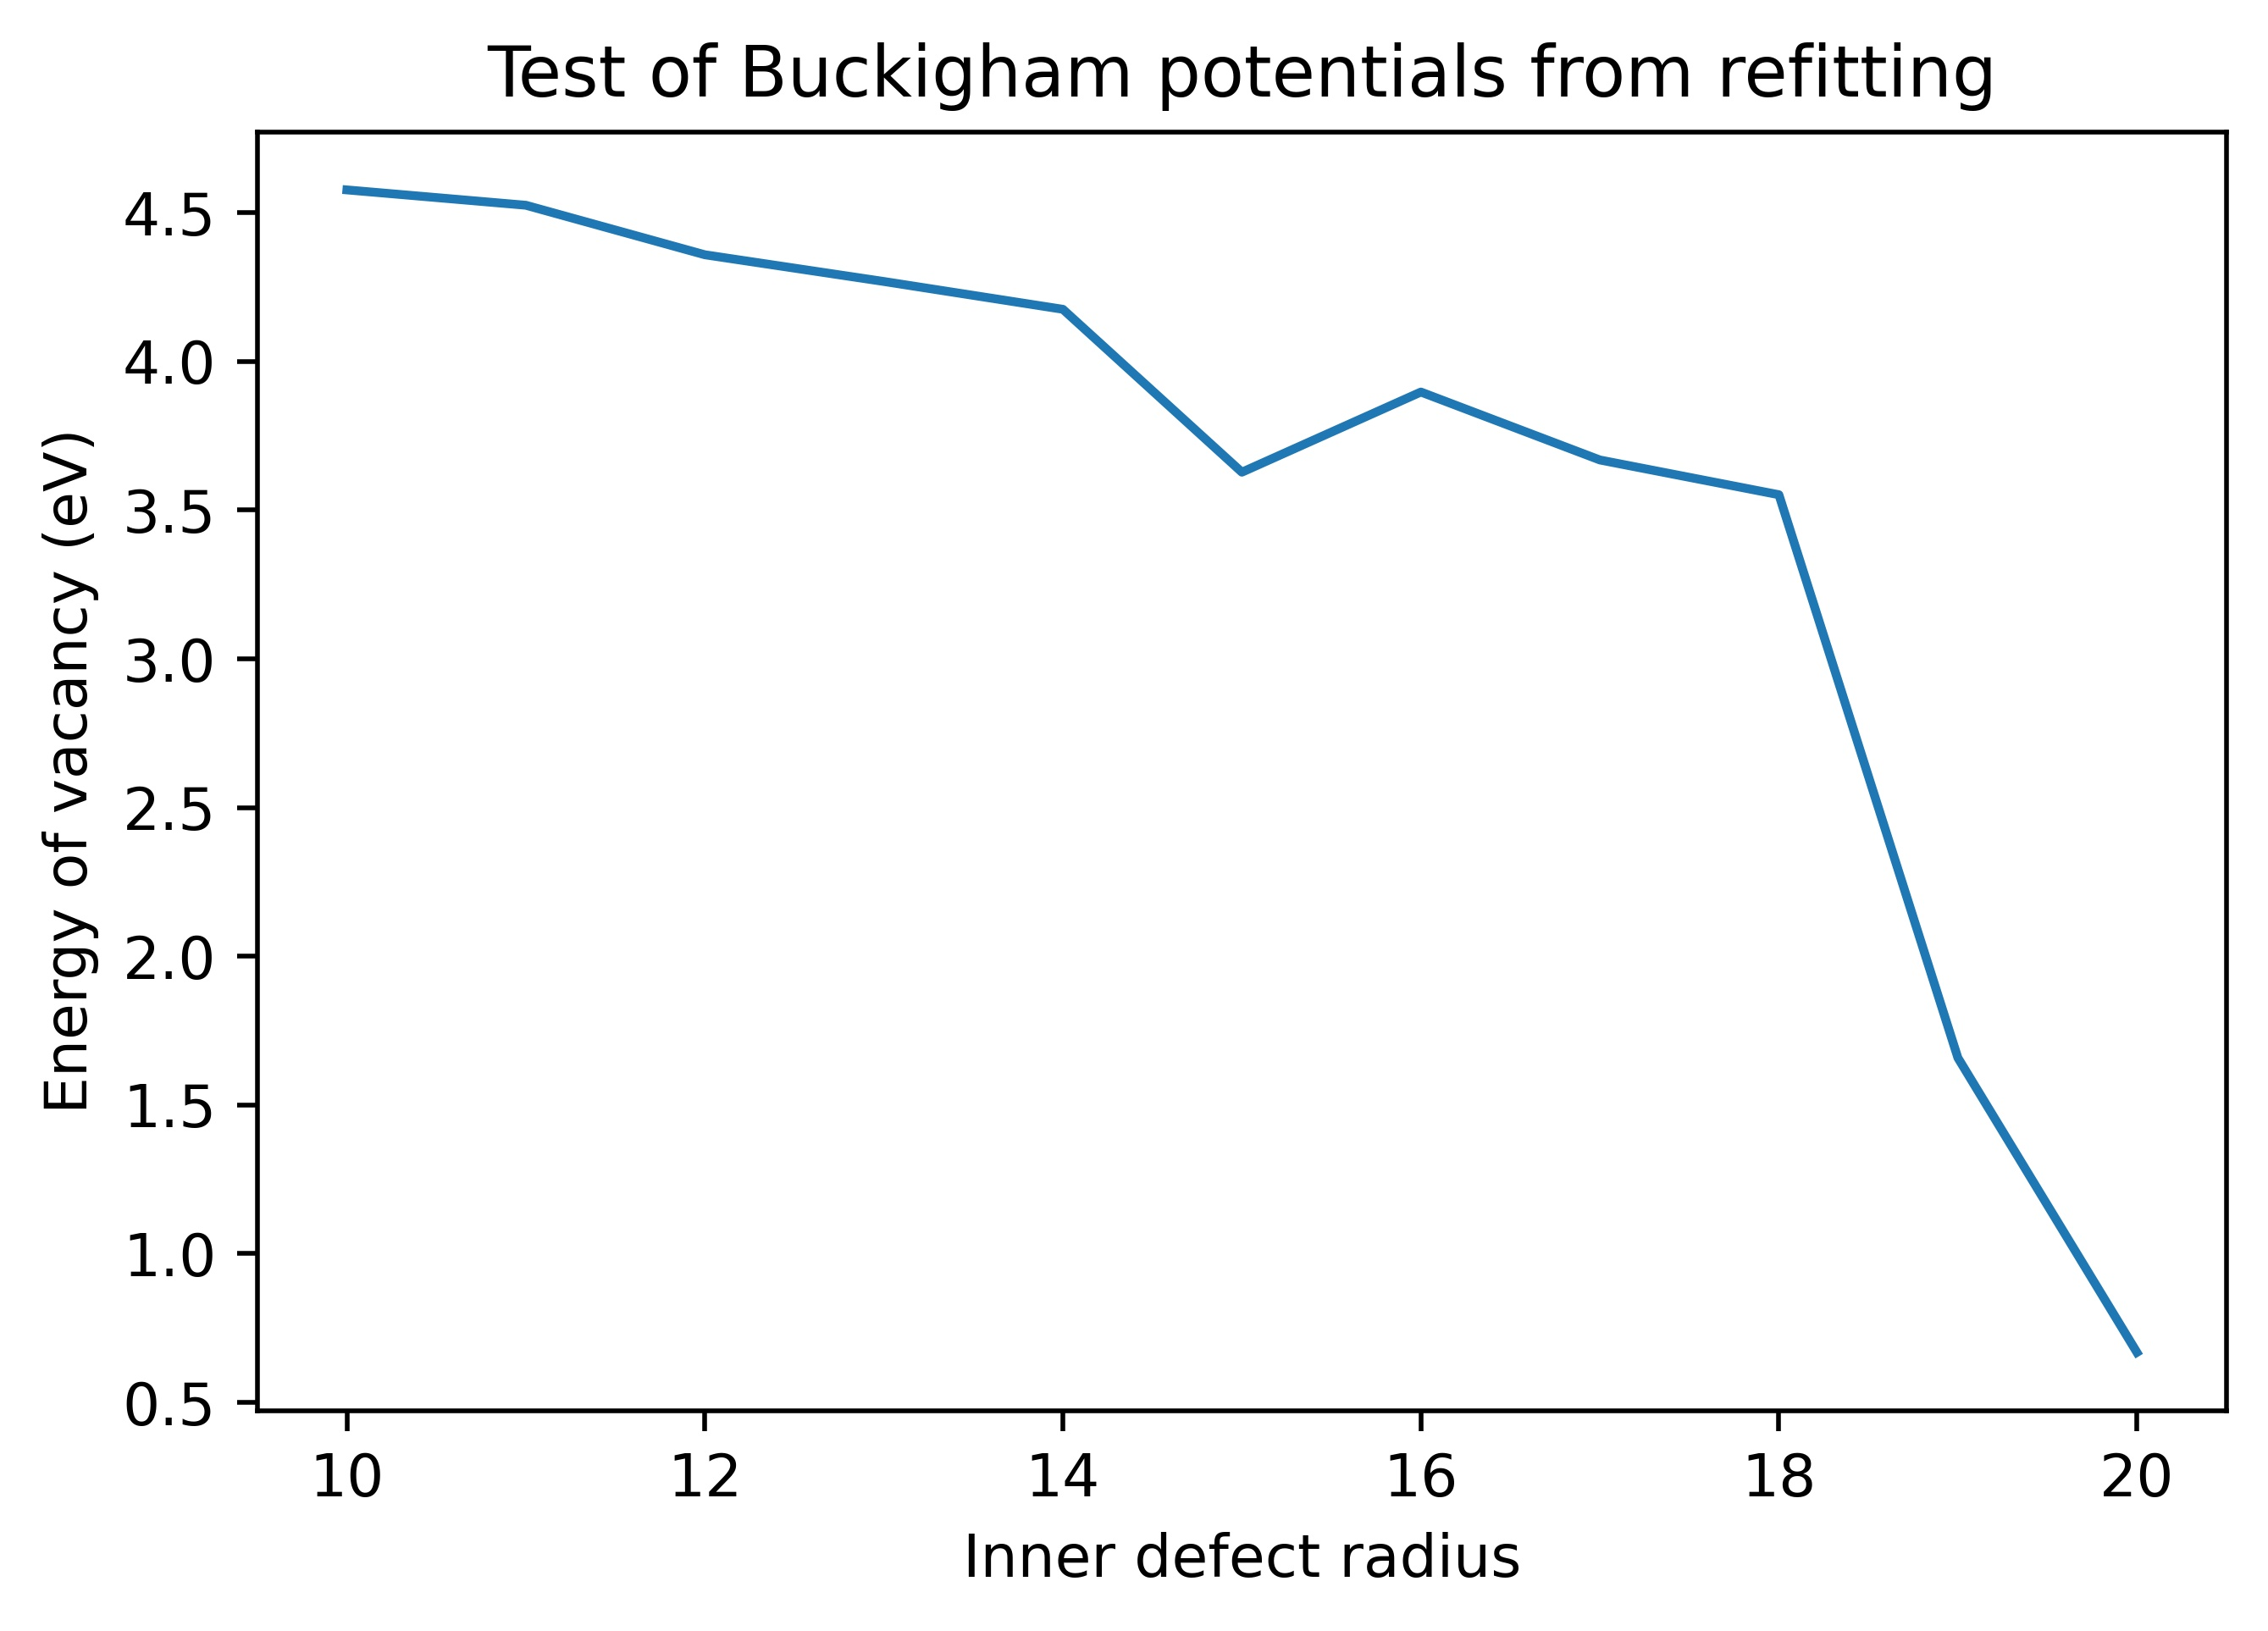
\includegraphics[width=0.5\textwidth]{/home/ben/Documents/gulp_calcs/0_summary/refitted_test.jpg}
\end{figure}

\begin{table}[h!]
  \begin{center}
    \caption{Buckingham potentials}
    \begin{tabular}{c|c|c}
      \hline
      Na-O & 1226.84 0.307 0 & 1225.11 0.307 0 \\
      Na-Cl & 2314.70 0.290 0 & 2292.53 0.290 0 \\
    \end{tabular}
  \end{center}
\end{table}

\end{frame}

\begin{frame}[shrink=10]
\frametitle{Literature search}

\begin{figure}[ht]
  \begin{minipage}{0.45\linewidth}
    \centering
      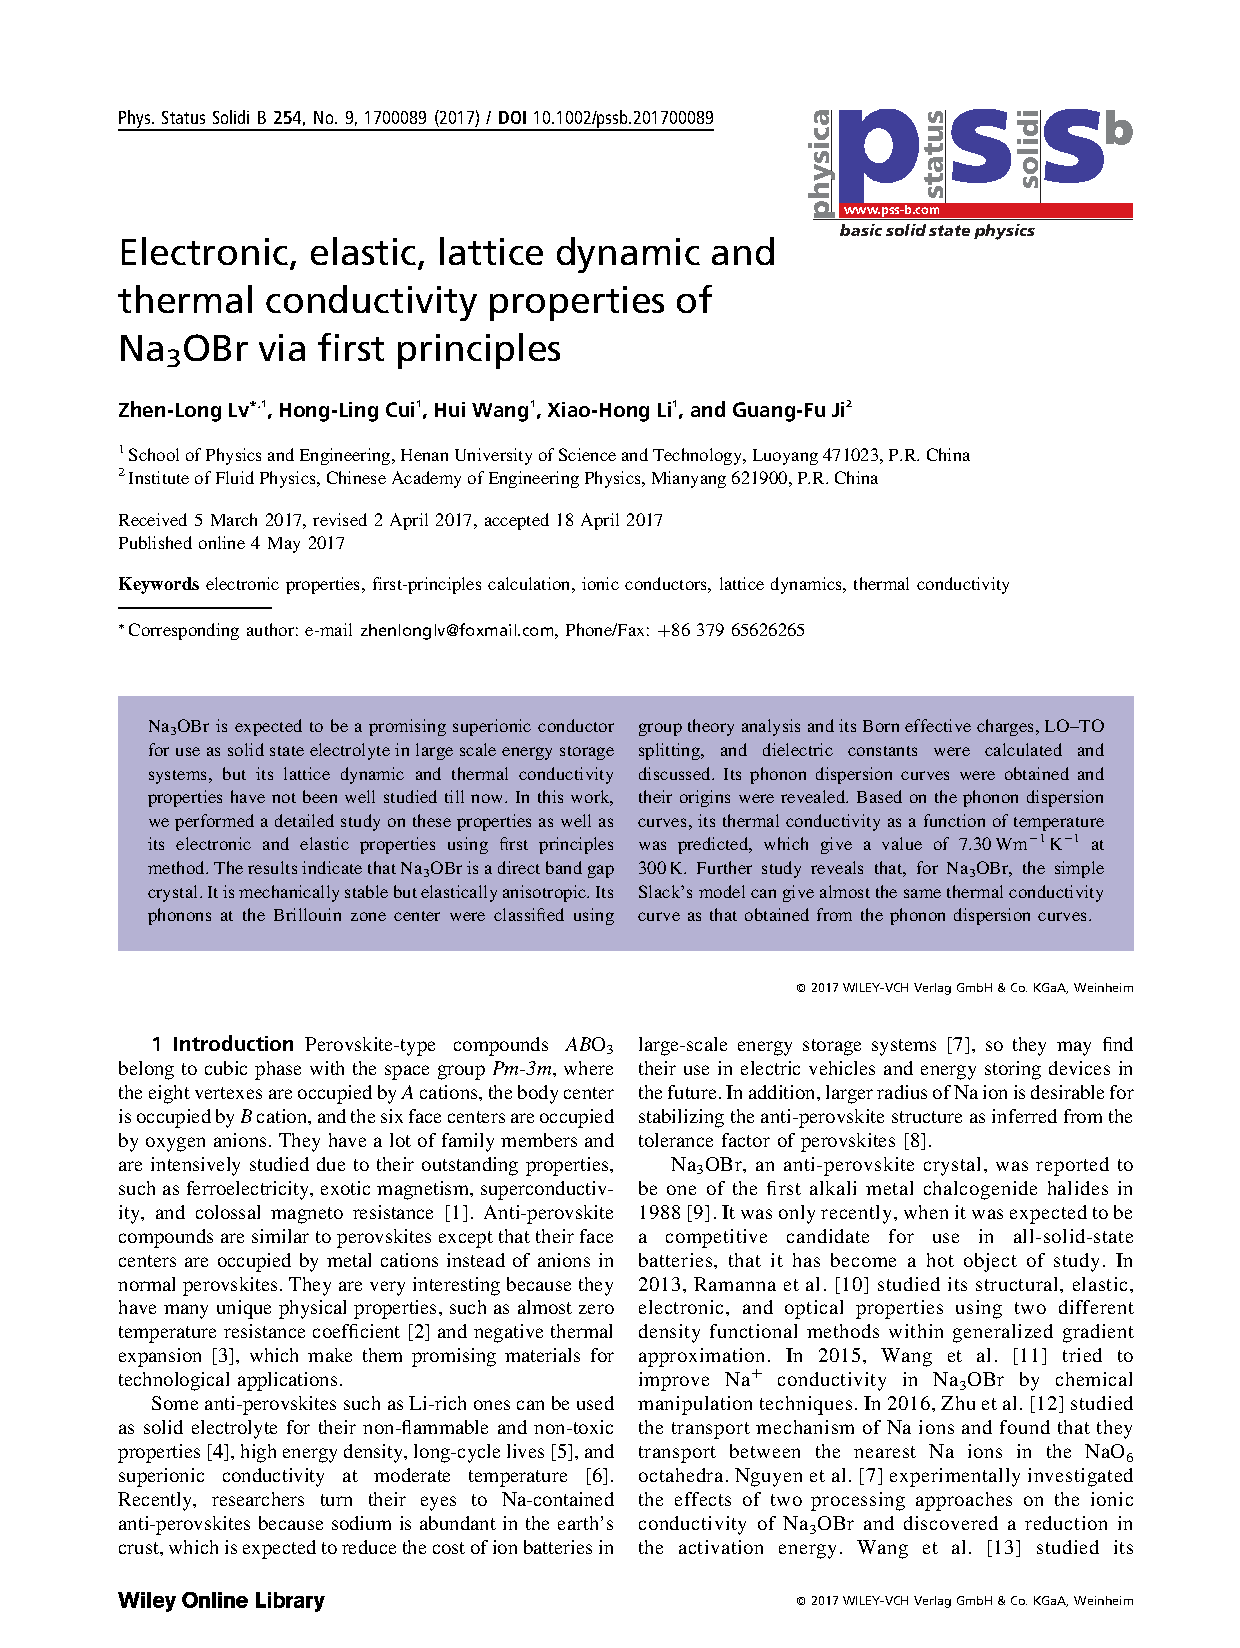
\includegraphics[width=\textwidth]{/home/ben/Pictures/Sattar2020.png}
      \caption{Sattar et al. (2020)}
      \includegraphics[width=\textwidth]{/home/ben/Pictures/Ramana2013.png}
      \caption{Ramana et al. (2013)}
  \end{minipage}
  \hspace{0.5cm}
  \begin{minipage}{0.45\linewidth}
    \centering
      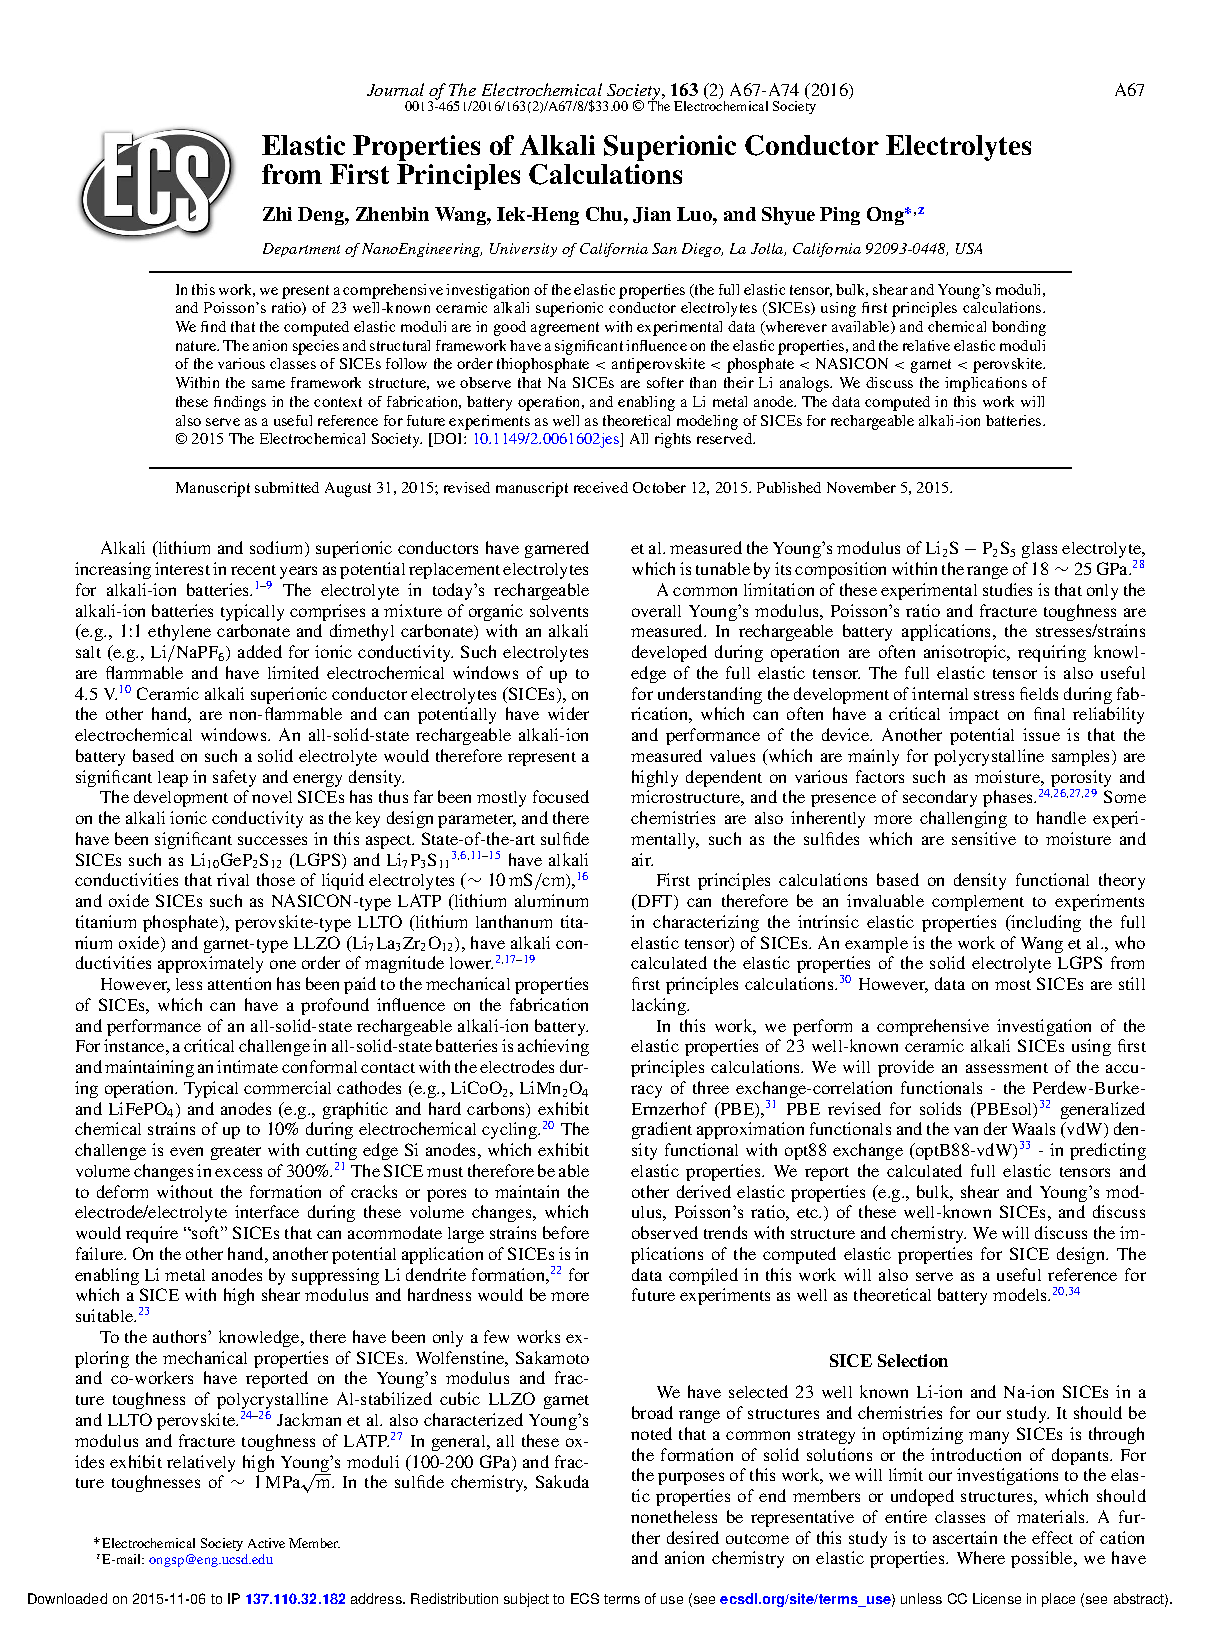
\includegraphics[width=\textwidth]{/home/ben/Pictures/Deng2016.png}
      \caption{Deng et al. (2016)}
      \includegraphics[width=\textwidth]{/home/ben/Pictures/Khandy2020.png}
      \caption{Khandy et al. (2020)}
  \end{minipage}
\end{figure}

\end{frame}

\begin{frame}[shrink=20]
\frametitle{Data used and potentials calculated}

\begin{table}[h!]
  \begin{center}
  \resizebox{\textwidth}{!}{%
    \begin{tabular}{l|c|c|c|c|c|c}
      \textbf{Paper} & \textbf{Model} & \textbf{Bulk, GPa} & \textbf{Shear, GPa} & \textbf{Na-O Buckingham} & \textbf{Na-Cl Buckingham} & \textbf{Variation} \\
      \hline
      Original & N/A & N/A & N/A & 1226.84 0.307 0 & 2314.70 0.290 0 & N/A \\
      Ramana2013 & FP-LAPW GGA & 32.5 & 21.9 & 322.01 0.388 0 & 1727.87 0.297 0 & 3.55 \\
      Ramana2013 & PW-PP GGA & 34.2 & 22.9 & 369.22 0.376 0 & 1775.12 0.300 0 & 0.58 \\
      Deng2016 & PAW GGA & 36.4 & 24.6 & 1042.96 0.310 0 & 1591.38 0.288 0 & 20.35 \\
      Khandy2020 & FP-LAPW GGA & 33.45 & 26.87 & 588.38 0.338 0 & 1170.41 0.315 0 & 0.04 \\
      Sattar2020 & FP-LAPW GGA & 32.53 & 25.42 & 477.56 0.354 0 & 1270.12 0.309 0 & 0.61 \\      
    \end{tabular}}
  \end{center}
\end{table}

\begin{figure}

\end{figure}
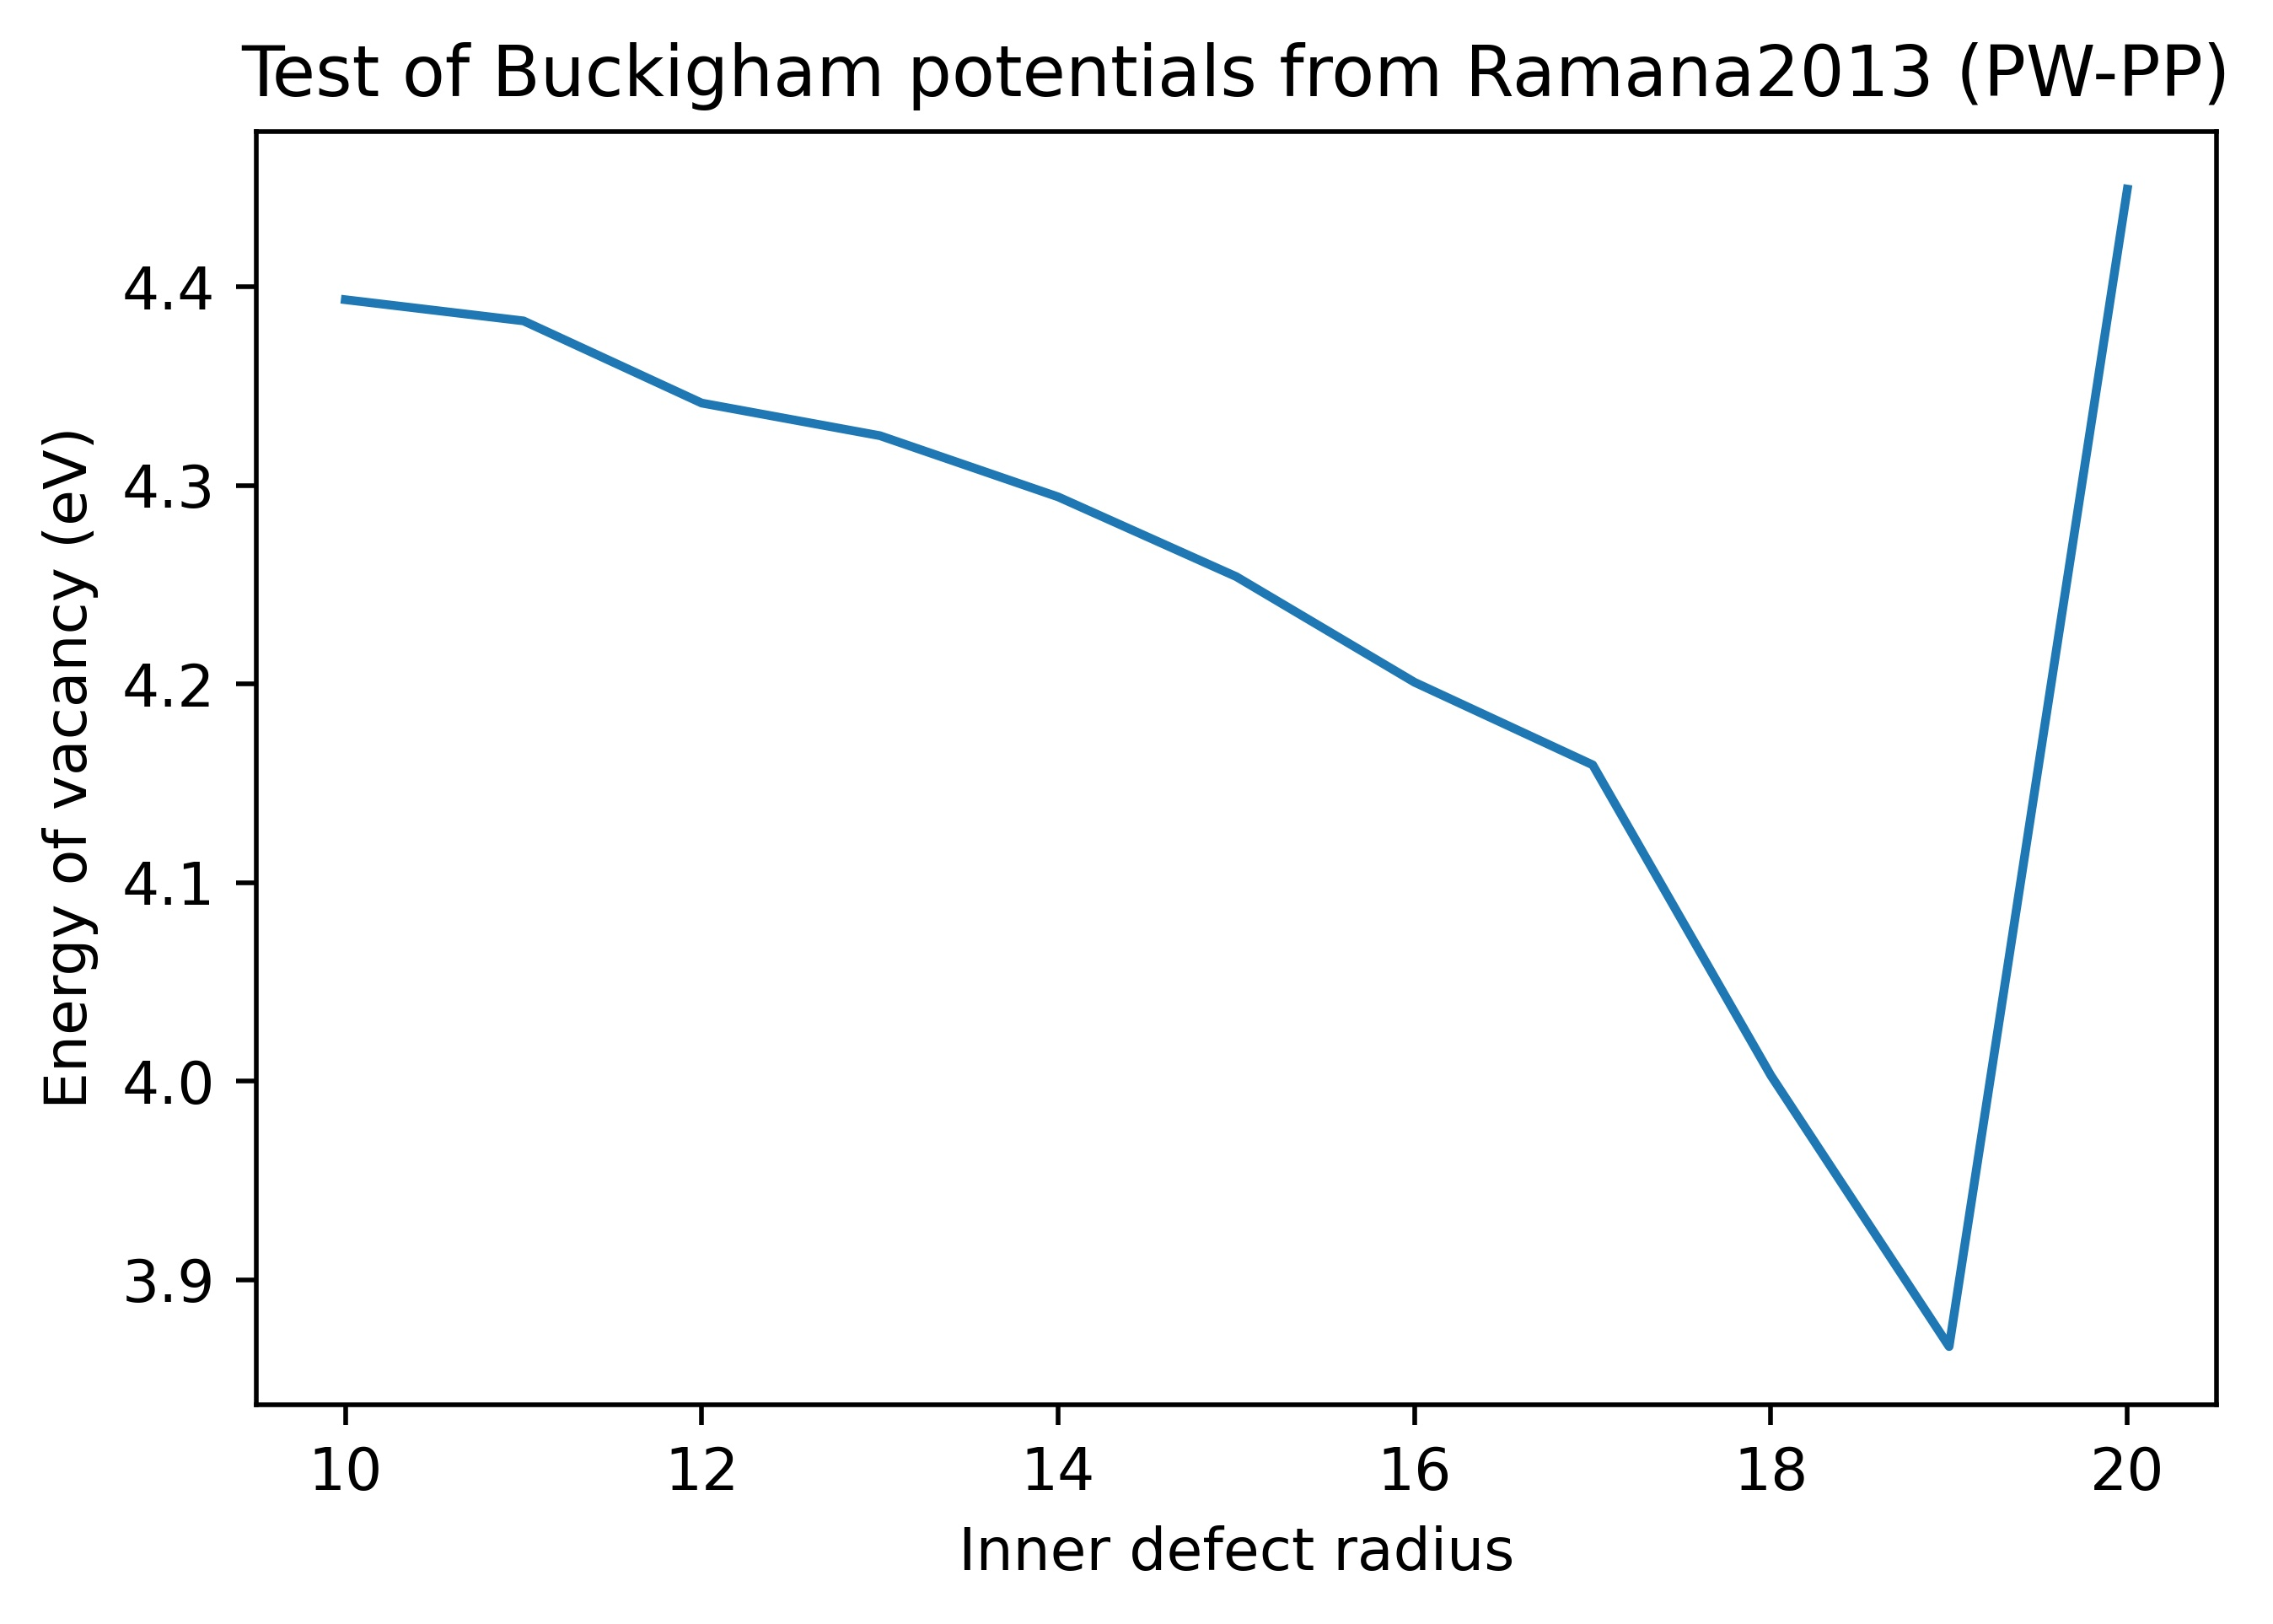
\includegraphics[width=0.33\textwidth]{/home/ben/Documents/gulp_calcs/0_summary/ramana_pwpp_test.jpg}%
\includegraphics[width=0.33\textwidth]{/home/ben/Documents/gulp_calcs/0_summary/khandy_test.jpg}%
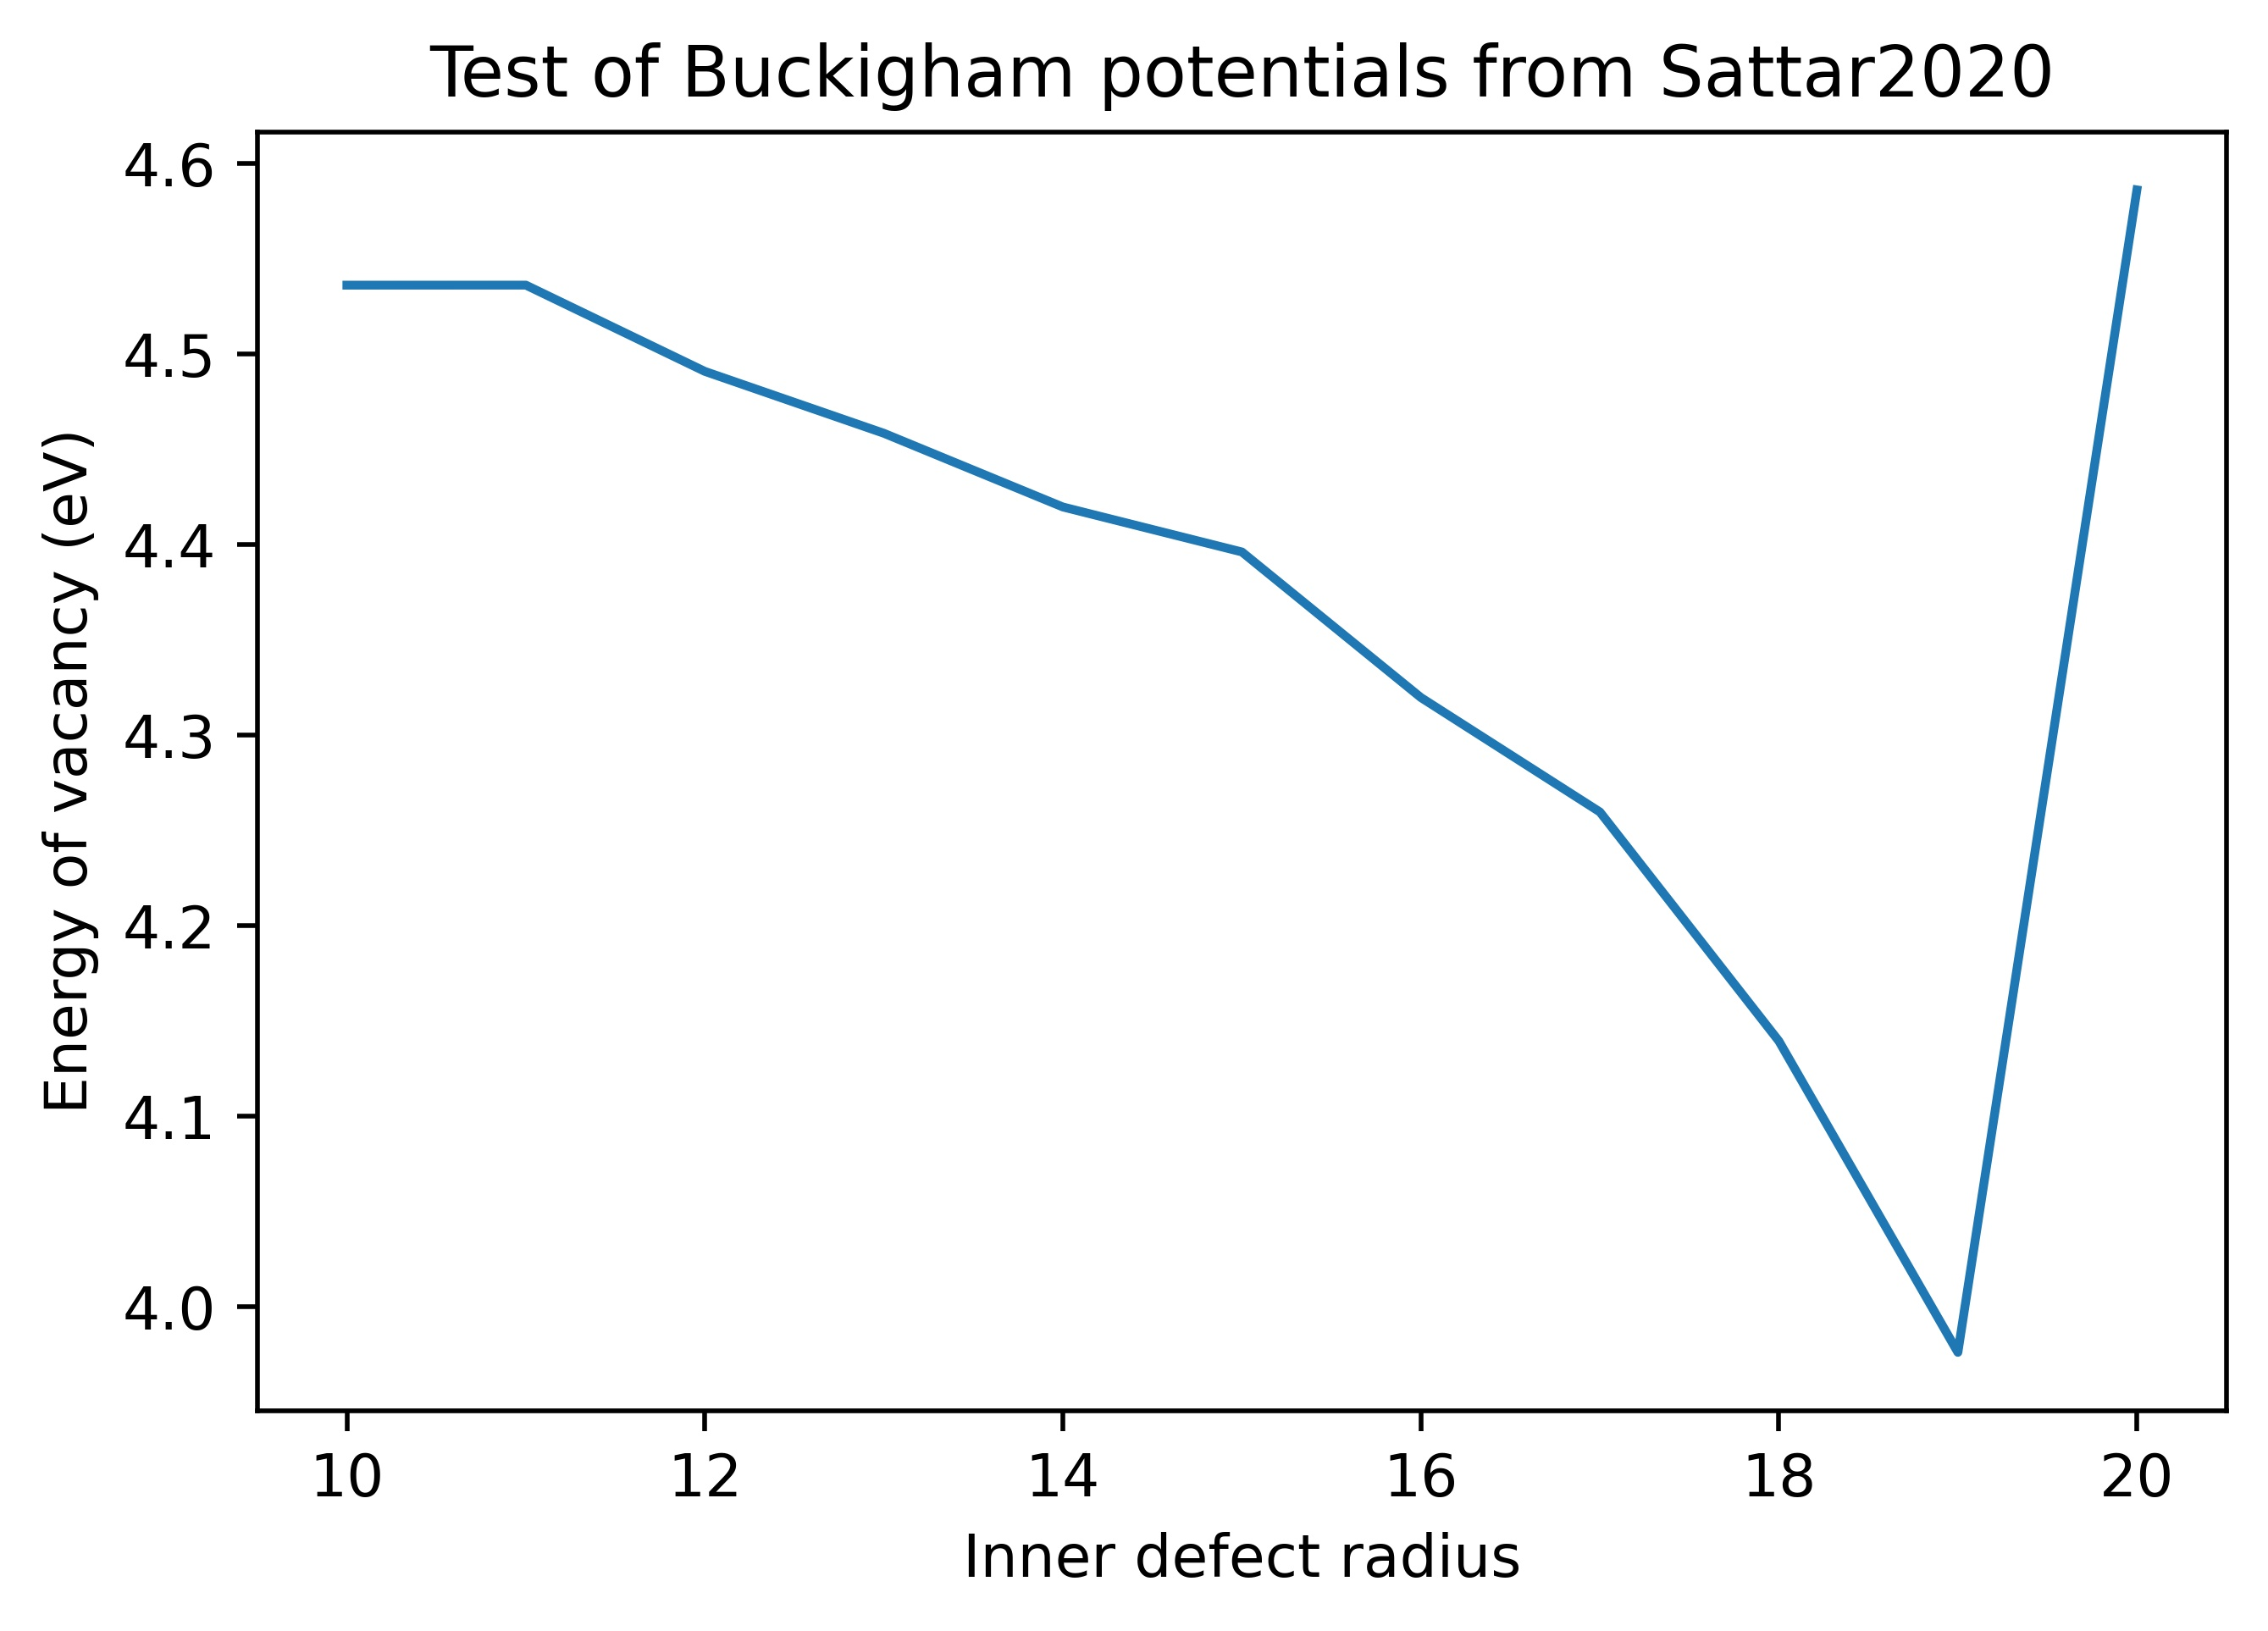
\includegraphics[width=0.33\textwidth]{/home/ben/Documents/gulp_calcs/0_summary/sattar_test.jpg}
\end{frame}

\begin{frame}
\frametitle{Comparison of Initial and Khandy potentials}

\begin{figure}
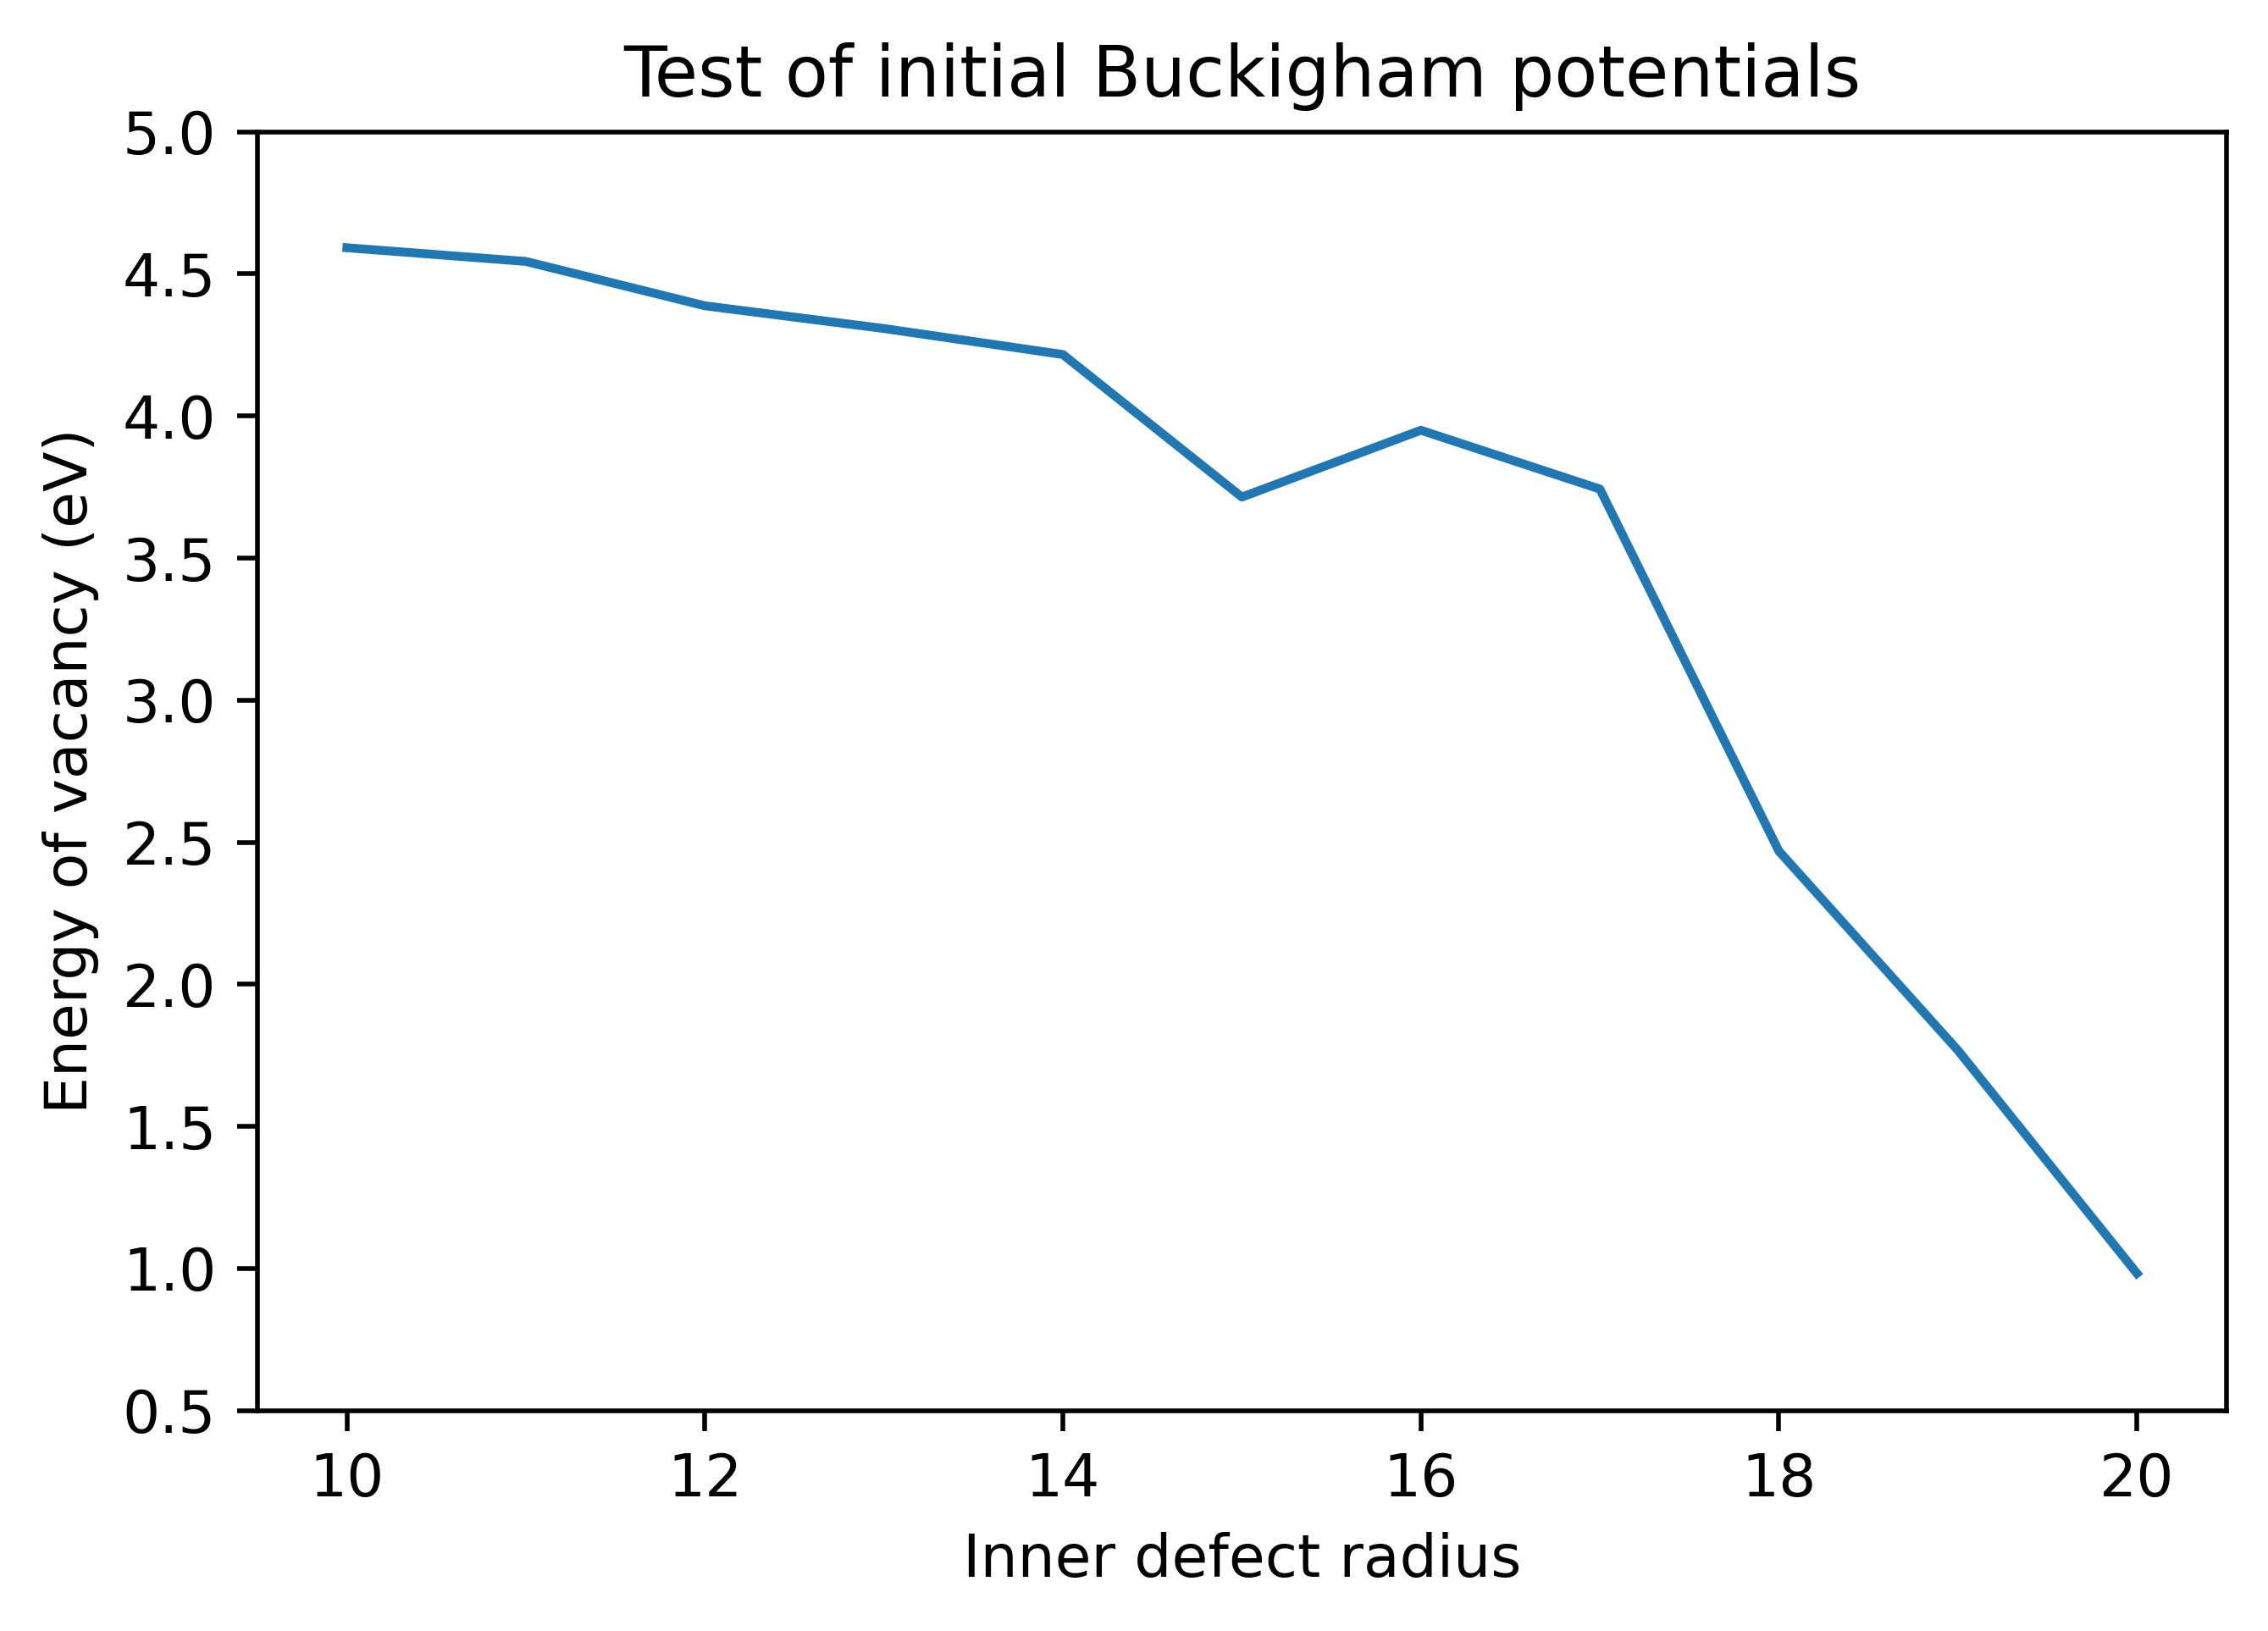
\includegraphics[width=0.5\textwidth]{/home/ben/Documents/gulp_calcs/0_summary/initial_test_scaled.jpg}%
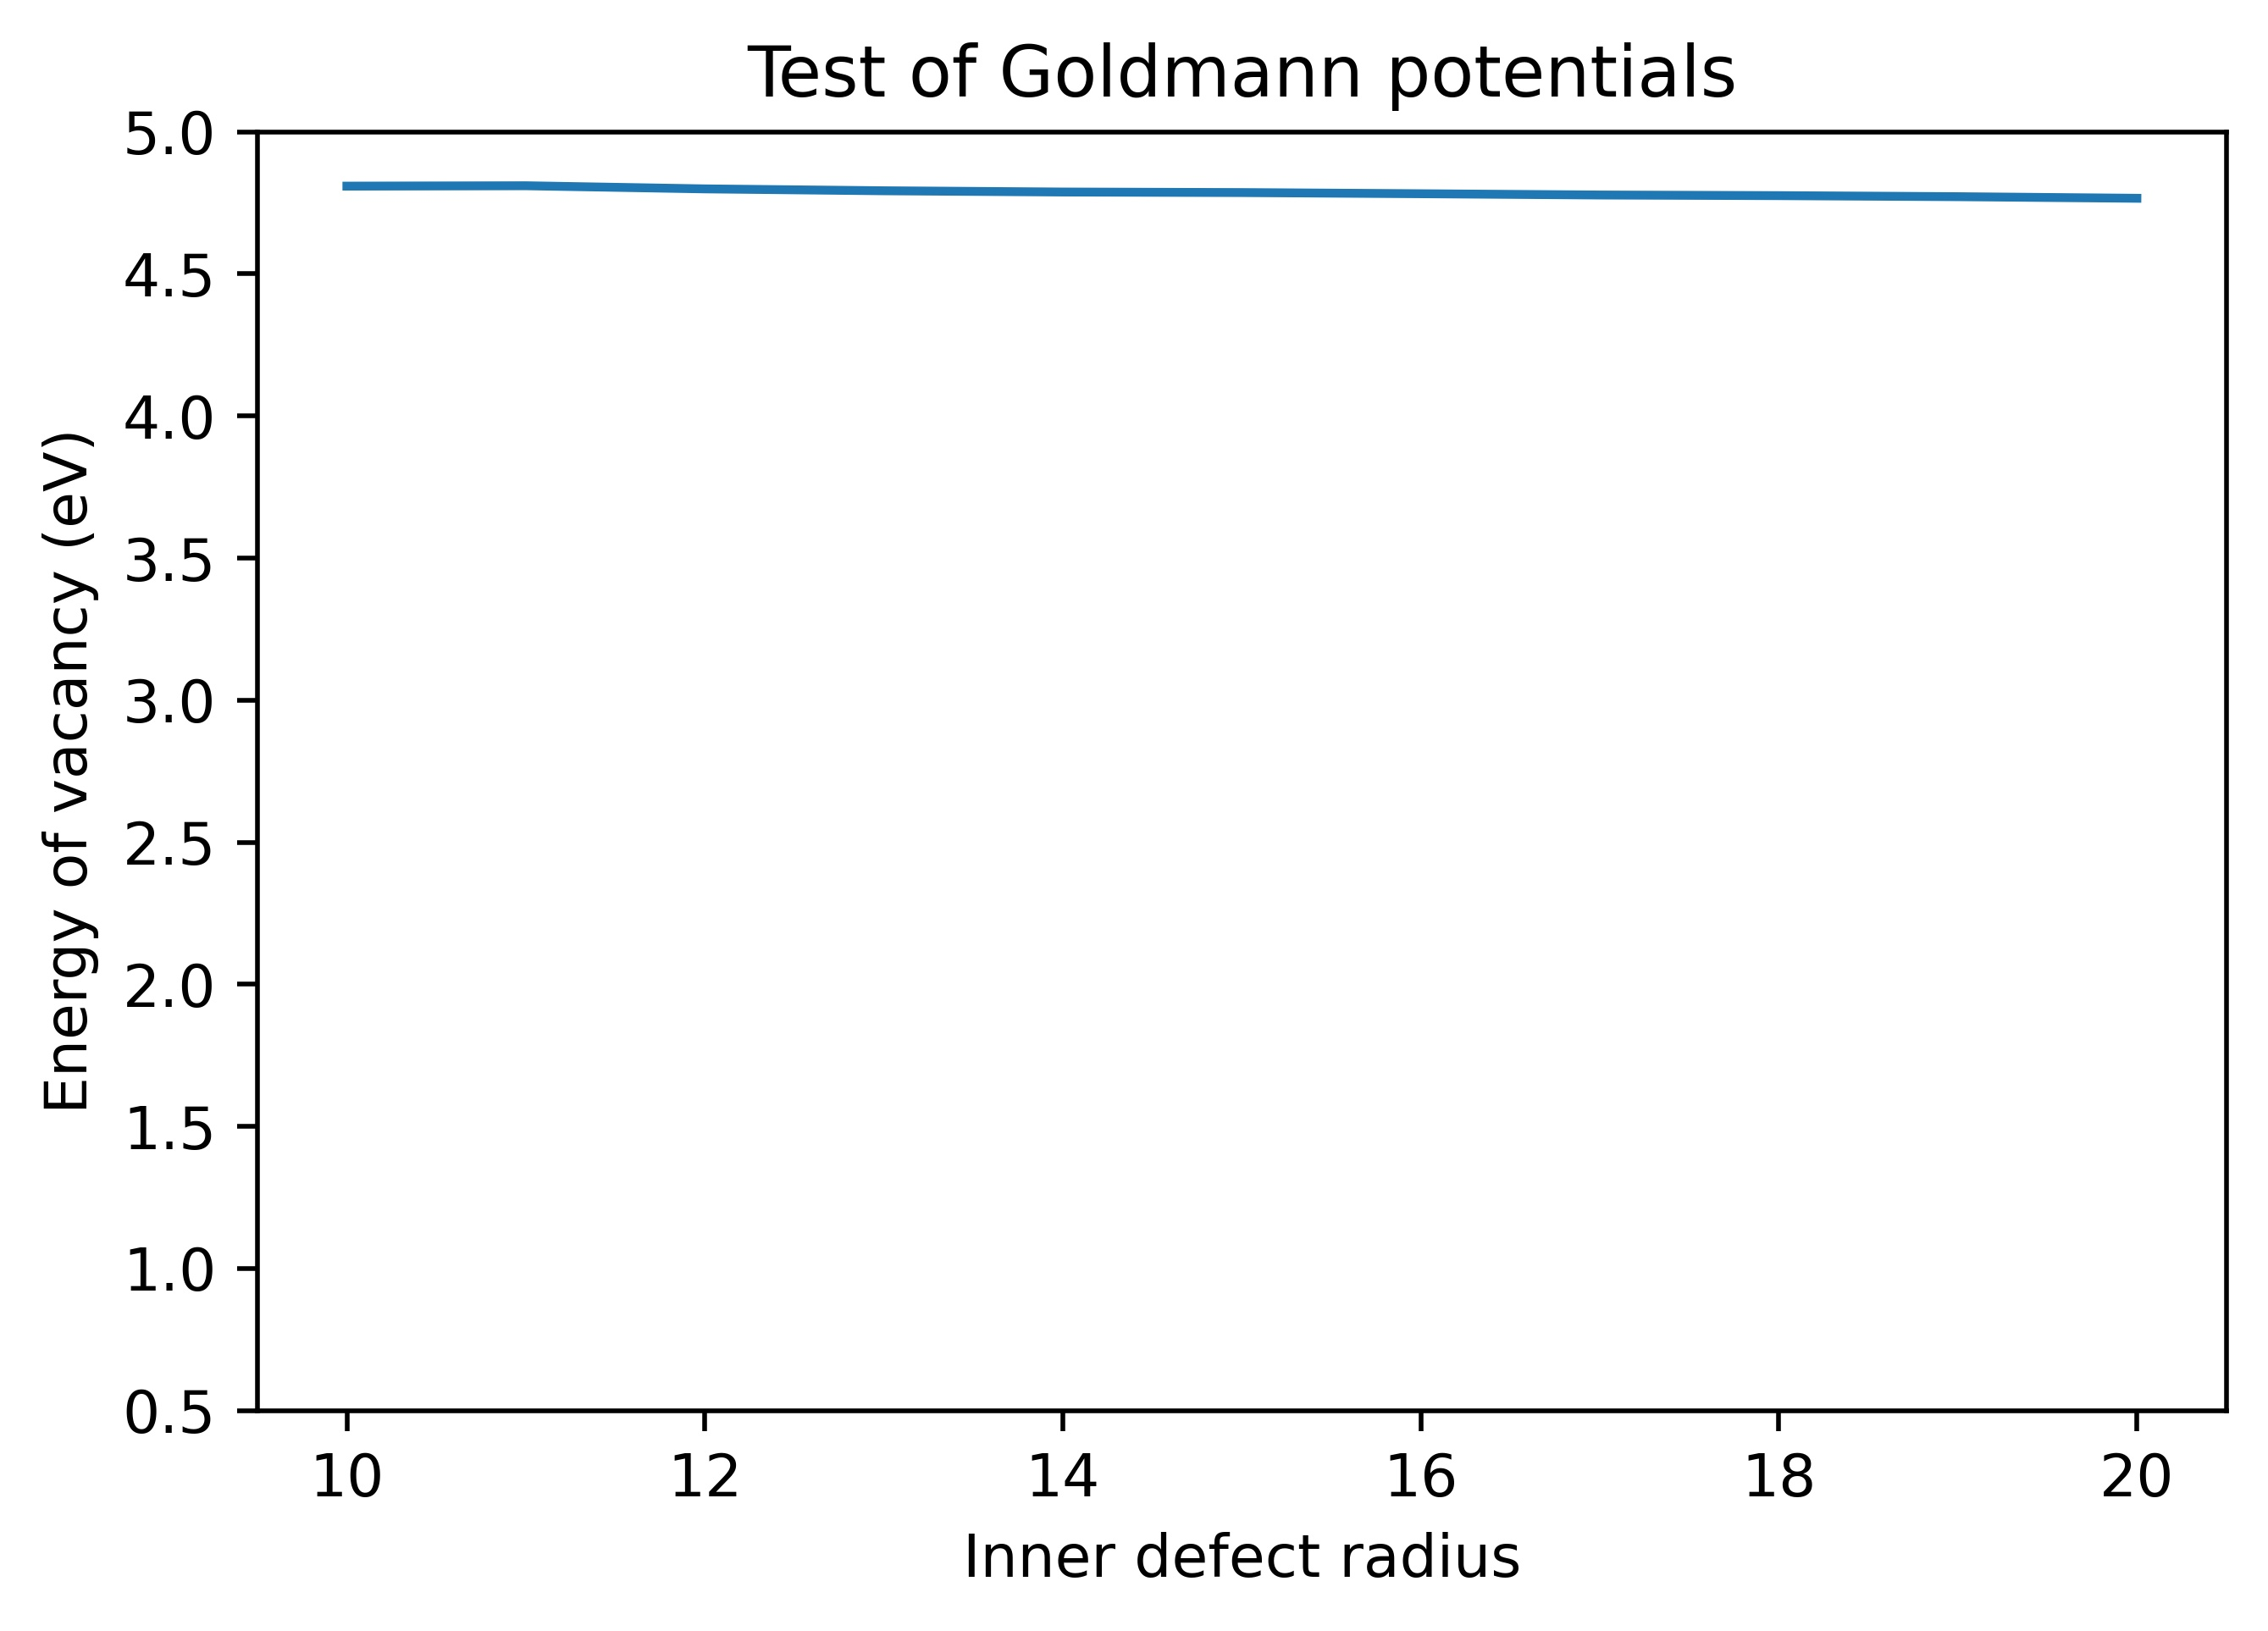
\includegraphics[width=0.5\textwidth]{/home/ben/Documents/gulp_calcs/0_summary/khandy_test_scaled.jpg}
\end{figure}

\end{frame}

\begin{frame}
\frametitle{Comparison of Initial and Khandy potentials}

\begin{figure}
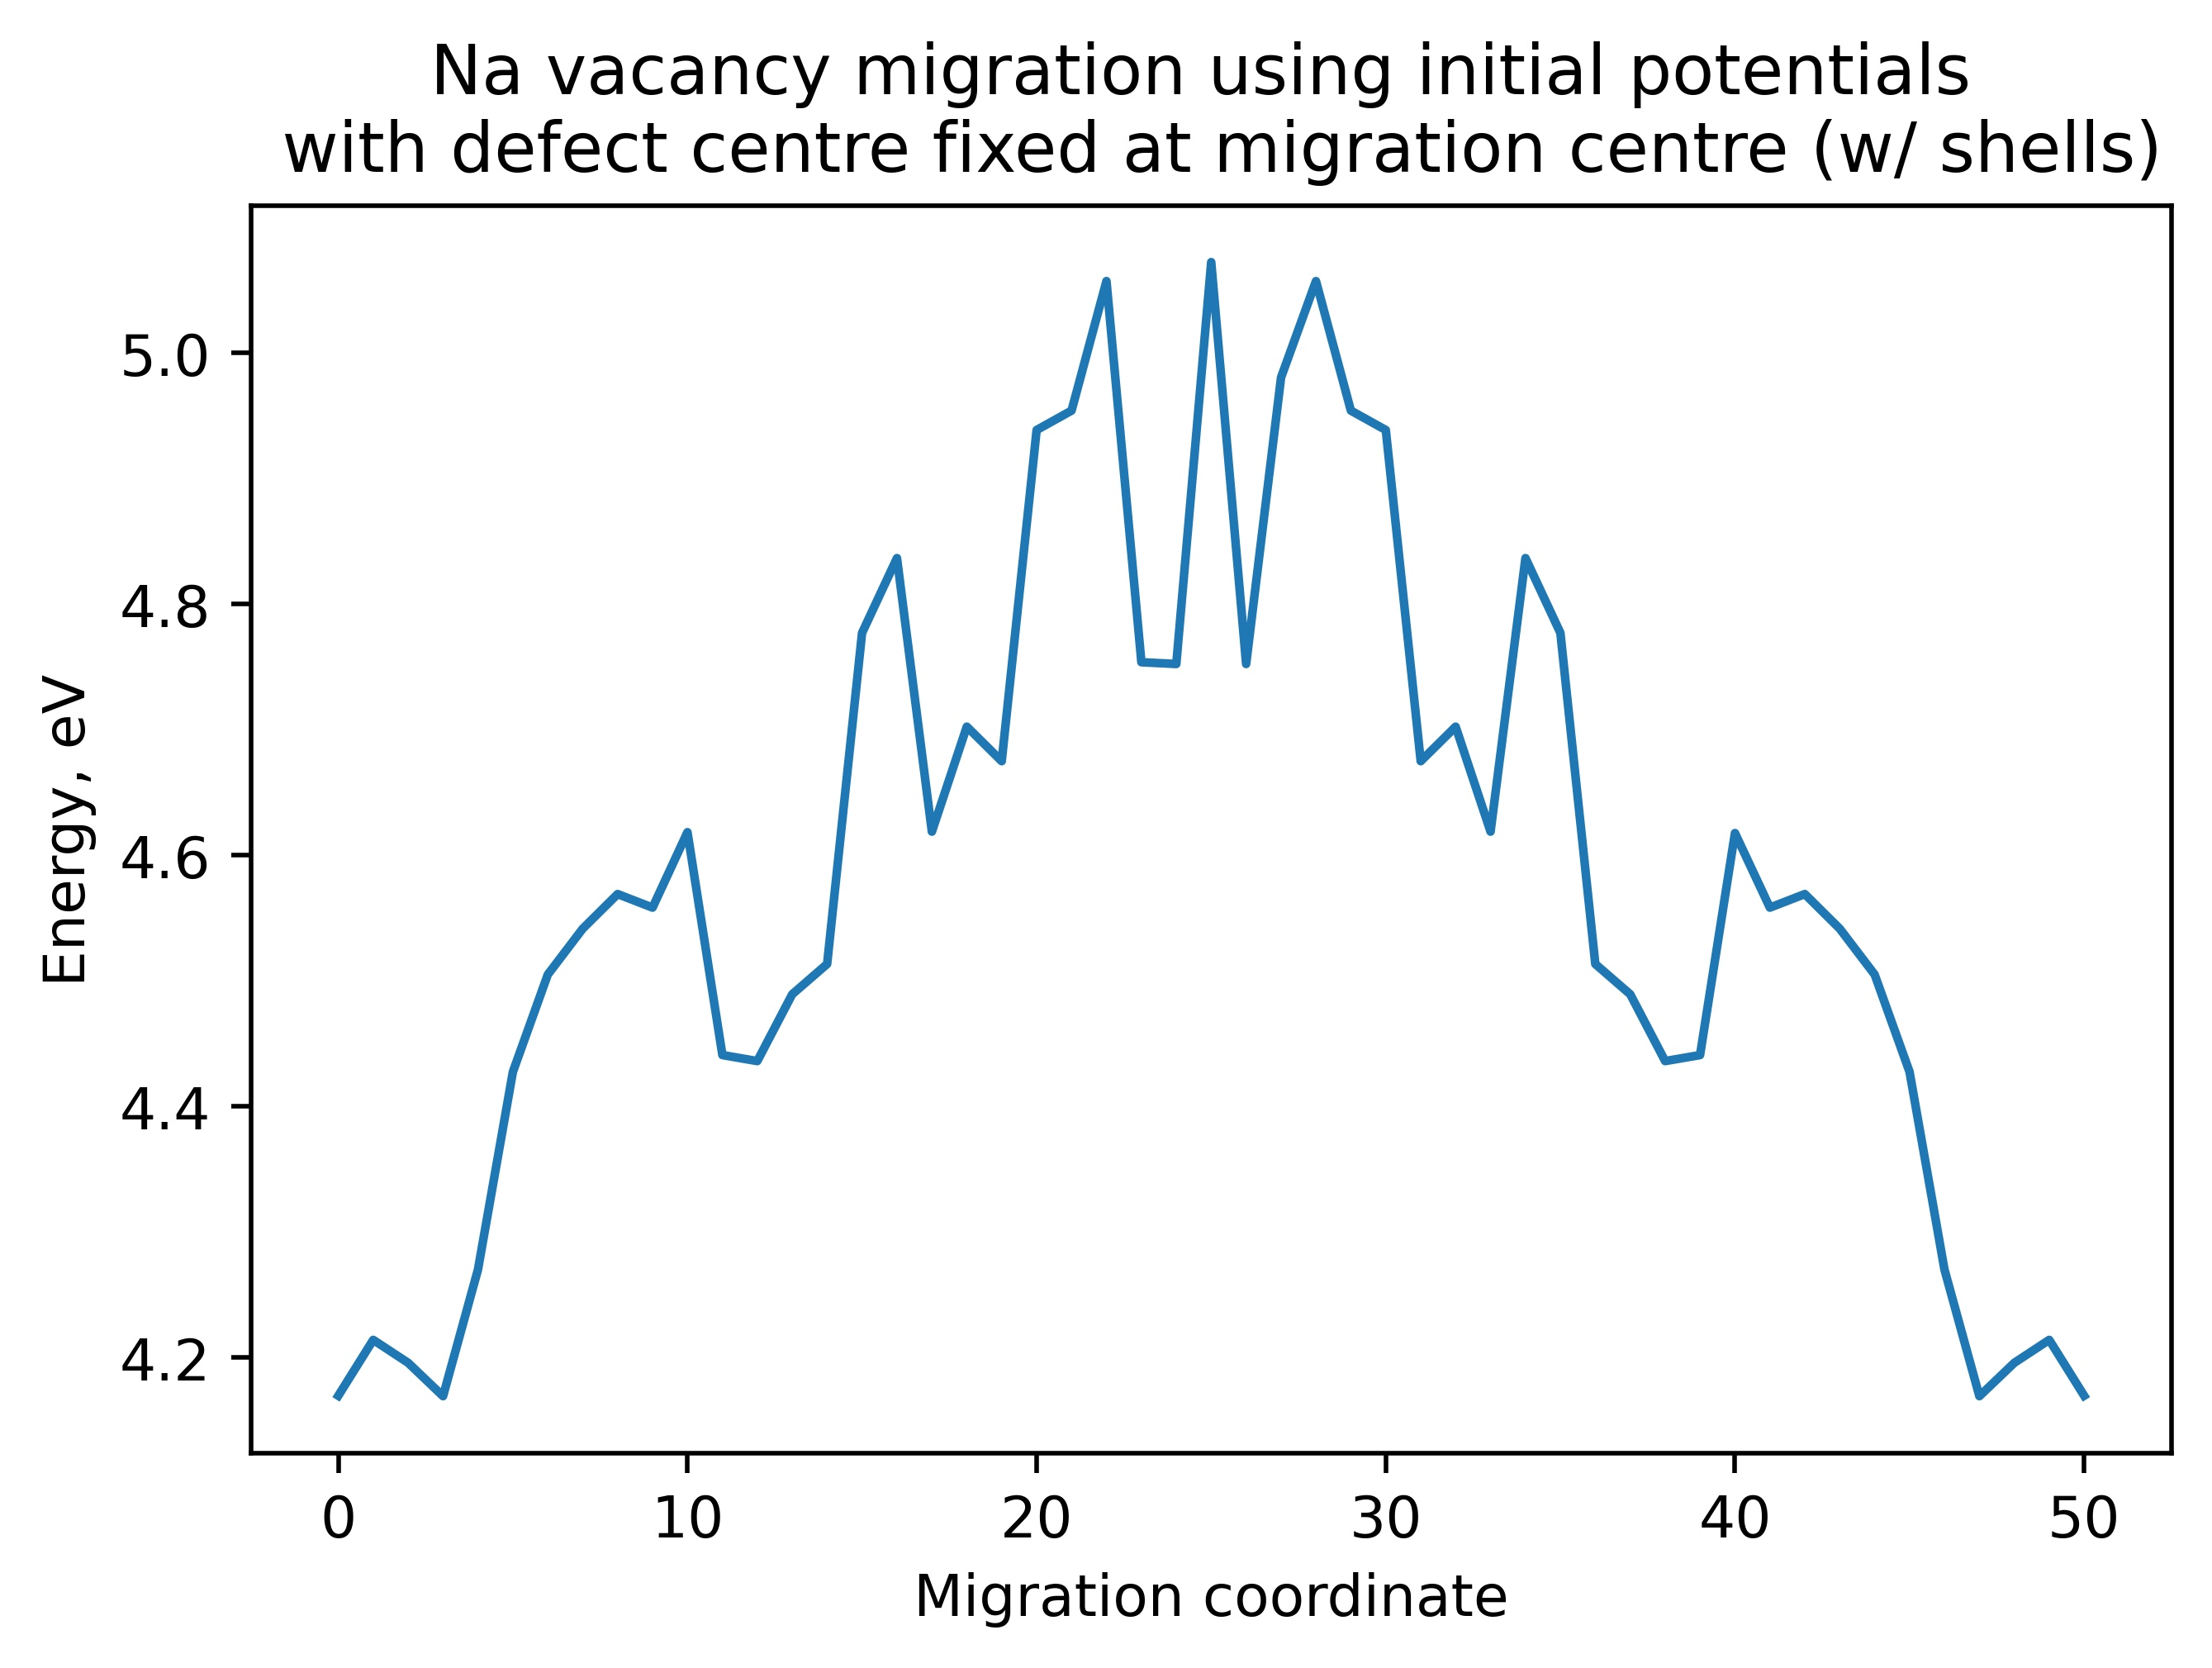
\includegraphics[width=0.5\textwidth]{/home/ben/Documents/gulp_calcs/0_summary/plot_na3ocl_fixcent_shel.jpg}%
\includegraphics[width=0.5\textwidth]{/home/ben/Documents/gulp_calcs/0_summary/khandy_migration_fixcent.jpg}
\end{figure}

\end{frame}

\begin{frame}
\frametitle{Calculations using potentials derived from Khandy2020}

\begin{table}[h!]
  \begin{center}
  \resizebox{\textwidth}{!}{%
    \begin{tabular}{l|c|c|c|c|c}
      \textbf{Parameter} & \textbf{Calc.} & \textbf{Comp. GGA} & \textbf{Comp. LDA} & \textbf{Comp. GULP} & \textbf{Experimental}\\
      \hline
      lattice parameter, $\AA$ & 4.41 & 4.54\cite{RN72}, 4.538\cite{RN78}, 4.53\cite{RN81}, 4.543\cite{RN82}, 4.514\cite{RN82}, 4.541\cite{RN84} & 4.382\cite{RN78}, 4.381\cite{RN82}, 4.31\cite{RN83} & 4.501\cite{RN55} & 4.504\cite{RN53}, 4.496\cite{RN69}, 4.500\cite{RN65}, 4.4908\cite{RN68} \\
      \hline
      Na Frenkel, eV & 2.58 & 1.94\cite{RN72}, 2.45\cite{RN55} & & \\
      NaCl Schottky, eV & 1.88 & 1.28\cite{RN72}, 1.75\cite{RN55} & & \\
      \ch{Na2O} Schottky, ev & 5.14 & 2.52\cite{RN72} & & \\
      \ch{Na3OCl} Schottky, ev & 6.74 & 6.10\cite{RN55} & & \\
      \hline
      Na vacancy migration, eV & 0.46 & 0.61\cite{RN72}, 0.428\cite{RN68}, 0.29\cite{RN53}, 0.29\cite{RN55} & & & 0.63\cite{RN68}, 1.04\cite{RN53} \\
    \end{tabular}}
  \end{center}
\end{table}

\begin{figure}
\includegraphics[width =7cm]{/home/ben/Documents/gulp_calcs/0_summary/bar_na3ocl_khandy_defects.jpg}
\end{figure}

\end{frame}

\begin{frame}
\frametitle{Review of results}

\begin{itemize}
  \item Concern over slightly off lattice parameter
  \item Discussion with Ben and Lucy
  \item They suggested that while the results may look good, they might not be accurate
  \item They proposed trying to fit the potentials using Lucy's code
  \item This involves thermally distorting the initial structure via AIMD, taking snapshots,, doing single-point calculations on the snapshots and fitting the potentials to them
\end{itemize}

\end{frame}

\begin{frame}[shrink=20]
\frametitle{Bibliography}

\bibliographystyle{rsc}
\bibliography{/home/ben/Documents/literature_review/exportlist}
\end{frame}

\end{document}